\subsection{Registrazione e indicizzazione delle varianti in etcd}
\label{sec:variant-registration}

Le varianti di una funzione logica vengono definite tramite un file 
JSON collocato nella directory \texttt{variants/<LogicalName>/} del 
progetto. Al momento della registrazione, il sistema legge questo file 
attraverso il componente \texttt{FileSource}, prepara il codice 
sorgente di ciascuna variante in formato tar e materializza le varianti 
in etcd attraverso la funzione \texttt{CreateInternalVariants}.

\subsubsection{Convenzione di denominazione}

La convenzione di denominazione distingue la variante di riferimento 
dalle varianti alternative. La prima variante definita nel file JSON, tipicamente quella a massima accuratezza, mantiene come nome interno 
esattamente il \texttt{LogicalName}, preservando la compatibilità con 
le invocazioni che non specificano alcuna preferenza energetica. Le 
varianti successive ricevono un nome composto nella forma 
\texttt{<LogicalName>-<VariantID>}. Per la funzione logica 
\texttt{fibonacci} (\autoref{lst:fibonacci-json}) ad esempio, i nomi interni assegnati sono:

\begin{itemize}
    \item \texttt{fibonacci} — variante base in Python
    \item \texttt{fibonacci-optimization-py} — variante ottimizzata 
    in Python
    \item \texttt{fibonacci-c} — variante compilata in C nativo
\end{itemize}

\subsubsection{Struttura delle chiavi in etcd}

Il sistema mantiene in etcd due livelli distinti di chiavi, ciascuno 
con una responsabilità specifica, come illustrato in 
Figura~\ref{fig:etcd-structure}.

Il primo livello, sotto il prefisso \texttt{/function/}, contiene una 
chiave per ogni variante registrata nel sistema, indipendentemente 
dalla funzione logica di appartenenza. Il valore associato è la 
serializzazione JSON completa della struttura \texttt{Function}, che 
include il runtime, il codice sorgente, il profilo energetico corrente 
e il modello di output. È su queste chiavi che il worker periodico 
scrive gli aggiornamenti del campo \texttt{InvocationJoule} ad ogni 
ciclo di raccolta.

Il secondo livello, sotto il prefisso 
\texttt{/index/logical/<LogicalName>/}, costituisce un indice che 
associa ciascun nome logico all'insieme delle sue varianti. La 
motivazione di questo indice è di natura prestazionale: poiché la 
selezione della variante avviene nel critical path della richiesta di 
invocazione, è necessario che lo scheduler possa recuperare 
rapidamente tutte le varianti di una funzione logica senza dover 
scorrere l'intero prefisso \texttt{/function/}, che contiene tutte 
le funzioni registrate nel sistema. Tramite l'indice, il recupero 
avviene con una singola query con prefisso su 
\texttt{/index/logical/<LogicalName>/}, restituendo esclusivamente le 
varianti della funzione richiesta e contenendo così la latenza 
introdotta dalla fase di selezione a runtime.

\begin{figure}[H]
    \centering
    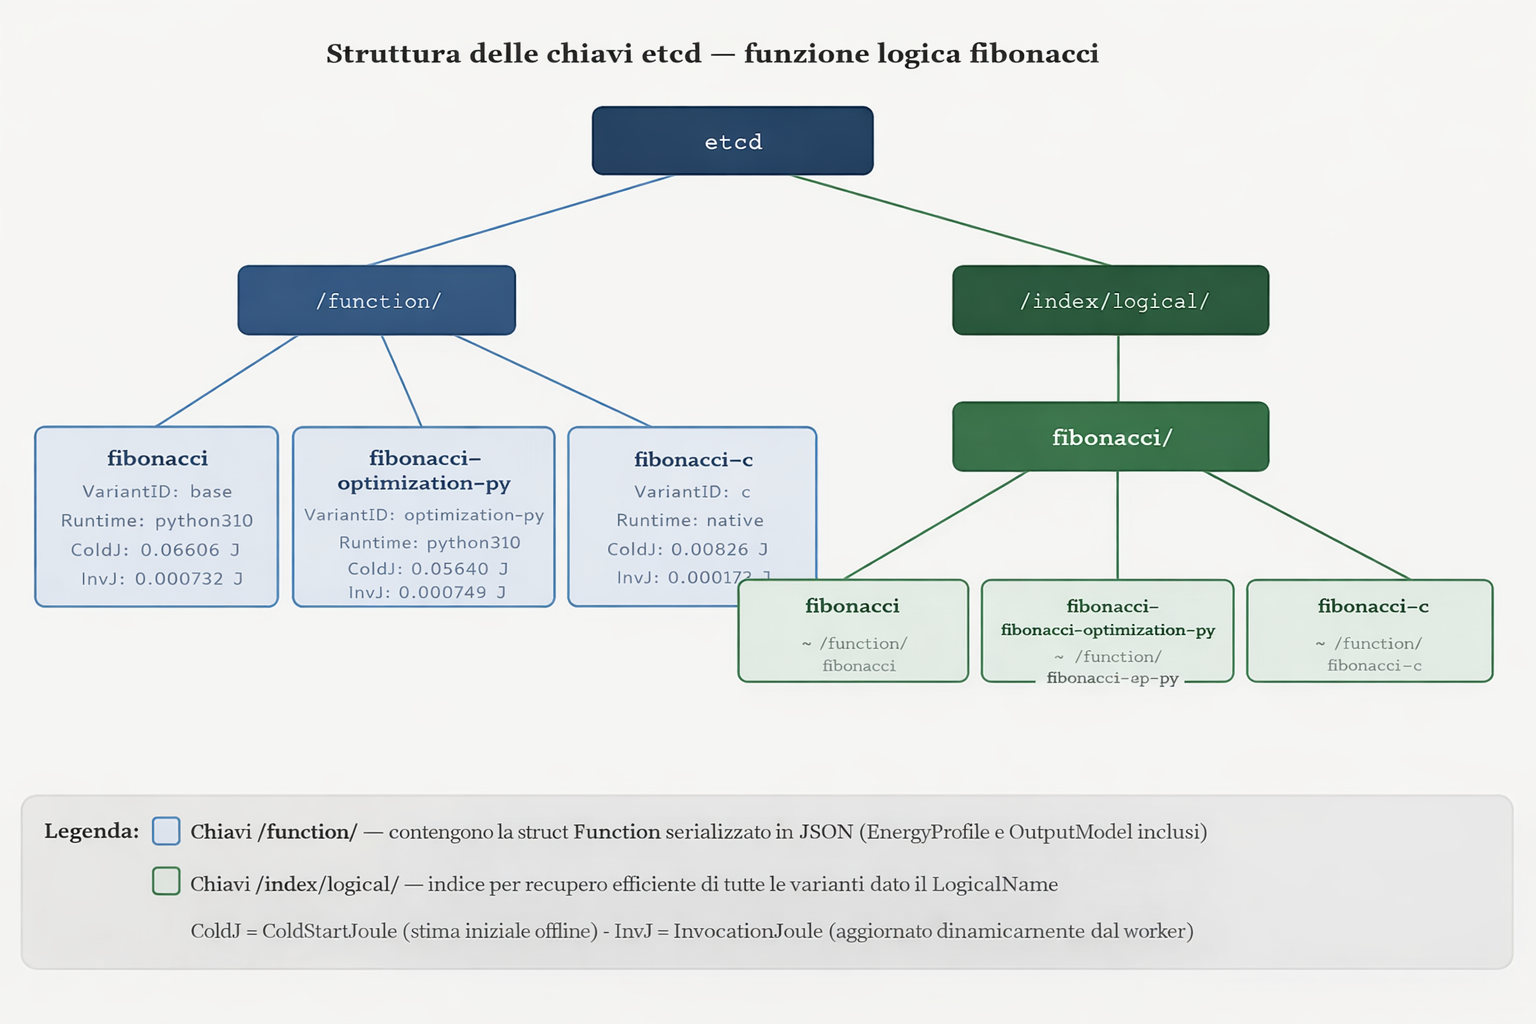
\includegraphics[width=0.95\textwidth]{figures/etcd-structure.jpg}
    \caption{Struttura delle chiavi etcd per la funzione logica 
    \texttt{fibonacci} con tre varianti. Le chiavi sotto 
    \texttt{/function/} contengono i profili completi aggiornati dal 
    worker periodico. L'indice sotto \texttt{/index/logical/} consente 
    allo scheduler di recuperare efficientemente le sole varianti della 
    funzione richiesta, senza scorrere l'intero store.}
    \label{fig:etcd-structure}
\end{figure}